% option draft um zu lange Zeilen anzuzeigen
\documentclass[a4paper,11pt]{book}

\usepackage[inner=3cm,outer=3cm]{geometry}
\usepackage[english]{babel}
\usepackage[utf8]{inputenc}
% linux libertine for normal text
\usepackage{libertine}
\usepackage{libertinust1math}
% inconsolate as teletype font
\usepackage{inconsolata}
\usepackage[T1]{fontenc}
\usepackage{color}
\usepackage{graphicx}
\usepackage{wrapfig}
\usepackage{amsmath}
\usepackage{amssymb}
\usepackage{mathastext}
\usepackage{subcaption}
\usepackage{pmboxdraw}
\usepackage{lipsum}
\usepackage[export]{adjustbox}
\usepackage{csquotes}
\usepackage{tabularx}
\usepackage[sort]{natbib}
\usepackage[toc,nonumberlist]{glossaries}
\usepackage{makecell}
\usepackage[absolute,overlay]{textpos}
\usepackage{microtype}
\usepackage[linesnumbered,ruled]{algorithm2e}
\usepackage[color]{register}
\usepackage[leftbars,color]{changebar}

\setlength{\changebarwidth}{.4em}

\colorlet{pemux}{blue!20}
\colorlet{vm}{red!20}
\colorlet{vmpex}{orange!40}

\newcommand{\extstart}[1]{\cbcolor{#1}\cbstart}
\newcommand{\extend}{\cbend}
\newcommand{\extbox}[1]{
  \begin{tikzpicture}
    \node[draw=black, fill=#1, minimum width=.3em, minimum height=.3em] {};
  \end{tikzpicture}
}

\renewcommand{\regBitWidth}{64}
\setlength{\regWidth}{\textwidth}

% setup of siunitx
\usepackage[binary-units=true]{siunitx}
\DeclareSIUnit{\bits}{bits}
\DeclareSIUnit{\cycle}{cycle}
\DeclareSIUnit{\cycles}{cycles}
\sisetup{
  list-final-separator = {, and },
  per-mode=symbol
}

% tikz
\usepackage{tikz}
\usepackage{tikz-uml}
\usetikzlibrary{arrows,automata,positioning}
\usetikzlibrary{shapes.geometric}
\usetikzlibrary{shapes.multipart}
\usetikzlibrary{arrows.meta}
\usetikzlibrary{calc}
\usetikzlibrary{intersections}
\usetikzlibrary{patterns}

% tikz setup
\usepackage{environ}
\makeatletter
\newsavebox{\measure@tikzpicture}
\NewEnviron{scaletikzpicturetowidth}[1]{%
  \def\tikz@width{#1}%
  \def\tikzscale{1}\begin{lrbox}{\measure@tikzpicture}%
  \BODY
  \end{lrbox}%
  \pgfmathparse{#1/\wd\measure@tikzpicture}%
  \edef\tikzscale{\pgfmathresult}%
  \BODY
}

\makeatother
\tikzstyle{thick arrow}=[-{Latex[length=2mm]}]

% hyperlinks
\usepackage{hyperref}
\hypersetup{
  pdfauthor   = {Nils Asmussen},
  pdftitle    = {TCU Specification},
  pdfborder   = {0 0 0 [0 0]},
  colorlinks  = false
}

% listings
\usepackage{listings}
\lstset{basicstyle=\small\ttfamily,breaklines=true}
\lstdefinestyle{myc++}{
  language=C++,
  morekeywords={size_t,ssize_t}
}

% ignore page group warnings
\pdfsuppresswarningpagegroup=1

% redefine some names
\addto\extrasenglish{%
  \renewcommand{\chapterautorefname}{Chapter}%
  \renewcommand{\sectionautorefname}{Section}%
  \renewcommand{\subsectionautorefname}{Section}%
  \renewcommand{\subsubsectionautorefname}{Section}%
}

% for smart references
\newcommand{\rref}[2][]{\autoref{#2}}

% names
\newcommand{\myos}{$\text{M}^\mathbf{3}$}
\newcommand{\myfs}{$\text{M}^\mathbf{3}$FS}

% TODOs
\newcommand{\todo}[1]{\fbox{\bfseries\sffamily\scriptsize\color{red}TODO: #1}}

\title{Trusted Communication Unit -- Specification}
\author{Nils Asmussen}
\date{\today}

\begin{document}

\maketitle
\tableofcontents

\chapter{System Overview}
\label{sec:systemoverview}

\newcommand{\fillpe}[3]{
    \node[below=.6em of pe#1.north] {#2};
    \node[cu, above right=.6em and .6em of pe#1.south west,#3] (cu#1) {CU};
    \node[tcu,above left=.6em and .6em of pe#1.south east,#3] (tcu#1) {TCU};

    \draw[noc] ($(pe#1.south west)-(0,1.0em)$) -- ($(pe3.south east)-(0,1.0em)$);
    \draw[noc] ($(pe#1.south west)-(0,1.2em)$) -- ($(pe3.south east)-(0,1.2em)$);
    \draw[noc] ($(pe#1.south west)-(0,1.4em)$) -- ($(pe3.south east)-(0,1.4em)$);

    \draw
      let \p1=(tcu#1.south), \p2=($(pe#1.south west)-(0,1.2em)$) in
      (tcu#1.south) -- (\x1, \y2);
    \fill[radius=.2em]
      let \p1=(tcu#1.south), \p2=($(pe#1.south west)-(0,1.2em)$) in
      (\x1, \y2) circle node {};
}

\begin{figure}[h]
  \center
  \begin{tikzpicture}[
      pe/.style={draw=gray,minimum width=9.5em,minimum height=8em},
      cu/.style={draw=gray,fill=red!50,minimum width=4.5em,minimum height=4.5em},
      tcu/.style={draw=gray,fill=green!50,minimum width=3em,minimum height=3em},
      noc/.style={draw=green},
    ]

    \node[pe] (pe1) {};
    \node[pe,right=2em of pe1] (pe2) {};
    \node[pe,right=2em of pe2] (pe3) {};

    \fillpe{1}{Kernel PE}{fill=green!50};
    \fillpe{2}{User PE}{};
    \fillpe{3}{User PE}{};

    \node[draw=black, fill=white,
          below right=.3em and .3em of cu2.north west,
          minimum width=3.9em, minimum height=3.9em] {App};

    \node[draw=black, fill=white,
          below right=.3em and .3em of cu3.north west,
          minimum width=1.8em, minimum height=1.8em] (app1) {\tiny App};
          \node[draw=black, fill=white,
          right=.3em of app1.east,
          minimum width=1.8em, minimum height=1.8em] (app2) {\tiny App};
    \node[draw=black, fill=white,
          above right=.3em and .3em of cu3.south west,
          minimum width=3.9em, minimum height=1.8em] (pex) {Priv};
    \node[draw=black, fill=pemux, above left=.3em and .3em of tcu3.south east] {};
    \node[draw=black, fill=vm, above left=.3em and 1.2em of tcu3.south east] {};

  \end{tikzpicture}
  \caption{System Overview.}
  \label{fig:sysoverview}
\end{figure}

\noindent The trusted communication unit~(TCU) is a building block that can be used to construct
secure systems. As shown in \rref{fig:sysoverview}, the system consists of multiple processing
elements~(PEs), each containing a compute unit~(CU) and a TCU. The PEs are linked through some
interconnect (e.g., a network-on-chip) and are split into \emph{kernel PEs} and \emph{user PEs}. The
former are privileged and manage the TCUs of the user PEs, whereas the latter are unprivileged.

In this system, the TCU, the interconnect, and the kernel PEs are trusted (shown green), whereas the
CUs in the user PEs are untrusted (shown red). By default, all PEs are isolated from each other, but
communication channels between PEs can be established. These communication channels can only be
establish by kernel PEs, but can be used afterwards by user PEs. Which PEs are kernel PEs is defined
by the TCU's \texttt{FEATURES} register. At boot, all PEs are kernel PEs, which can be changed by
the kernel booting on one specific PE before the other PEs start.

User PEs can have different complexities, mostly driven by the used CU. The left user PE uses a
simple core with scratchpad memory and a basic TCU without extensions. The right user PE uses a
complex core with caches and virtual memory support and a multiplexer (Priv) that supports multiple
applications on the same PE. These features require TCU extensions for virtual memory (\extbox{vm})
and PE sharing (\extbox{pemux}). This specification highlights the portions that are required by
only one extension in its color and portions that are required by either extension as
\extbox{vmpex}.

\section{Processing Elements}

\begin{figure}[h]
  \center
  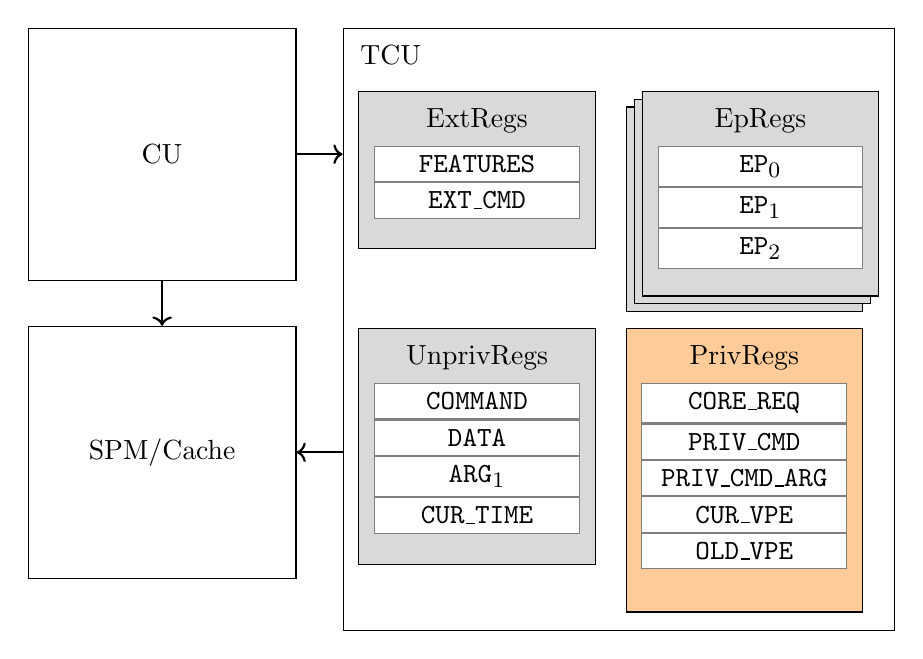
\begin{tikzpicture}[
      tcureg/.style={draw=gray,fill=white,minimum width=2.6cm},
      regtbl/.style={draw=black,fill=gray!30,minimum width=3cm}
    ]

    \node[draw=black,minimum width=7cm,minimum height=7.65cm,anchor=north west] (tcu) at(4,0) {};
    \node[draw=black,minimum width=3.4cm,minimum height=3.2cm,anchor=north west] (cu) at (0,0) {CU};
    \node[draw=black,minimum width=3.4cm,minimum height=3.2cm,anchor=south west] (mem) at (0,-7) {SPM/Cache};

    \node[below right=.1cm and .1cm of tcu.north west] {TCU};

    \node[
      regtbl,below right=.8cm and .2cm of tcu.north west,minimum height=2cm
    ] (tcuregs) {};
    \node[below=.1cm of tcuregs.north] {ExtRegs};
    \node[tcureg,below=.7cm of tcuregs.north] (extreg0) {\texttt{FEATURES}};
    \node[tcureg,below=0cm of extreg0]        (extreg1) {\texttt{EXT\_CMD}};

    \node[
      regtbl,below=1cm of tcuregs.south,minimum height=3cm
    ] (cmdregs) {};
    \node[below=.1cm of cmdregs.north] {UnprivRegs};
    \node[tcureg,below=.7cm of cmdregs.north] (cmdreg0) {\texttt{COMMAND}};
    \node[tcureg,below=0cm of cmdreg0]        (cmdreg1) {\texttt{DATA}};
    \node[tcureg,below=0cm of cmdreg1]        (cmdreg2) {\texttt{ARG$_1$}};
    \node[tcureg,below=0cm of cmdreg2]        (cmdreg3) {\texttt{CUR\_TIME}};

    \node[
      regtbl,below left=1cm and .4cm of tcu.north east,minimum height=2.6cm
    ] {};
    \node[
      regtbl,below left=.9cm and .3cm of tcu.north east,minimum height=2.6cm
    ] {};
    \node[
      regtbl,below left=.8cm and .2cm of tcu.north east,minimum height=2.6cm
    ] (epregs) {};
    \node[below=.1cm of epregs.north] {EpRegs};
    \node[tcureg,below=.7cm of epregs.north] (epreg0) {\texttt{EP$_0$}};
    \node[tcureg,below=0cm of epreg0]        (epreg1) {\texttt{EP$_1$}};
    \node[tcureg,below=0cm of epreg1]        (epreg2) {\texttt{EP$_2$}};

    \node[
      regtbl,fill=vmpex,below right=0cm and .38cm of cmdregs.north east,minimum height=3.6cm
    ] (prvregs) {};
    \node[below=.1cm of prvregs.north] {PrivRegs};
    \node[tcureg,below=.7cm of prvregs.north] (prvreg0) {\texttt{CORE\_REQ}};
    \node[tcureg,below=0cm of prvreg0]        (prvreg1) {\texttt{PRIV\_CMD}};
    \node[tcureg,below=0cm of prvreg1]        (prvreg2) {\texttt{PRIV\_CMD\_ARG}};
    \node[tcureg,below=0cm of prvreg2]        (prvreg3) {\texttt{CUR\_VPE}};
    \node[tcureg,below=0cm of prvreg3]        (prvreg4) {\texttt{OLD\_VPE}};

    \path
      let \p1=(cu.east), \p2=(tcu.west) in
      [draw=black,thick,->] (cu.east) -- (\x2,\y1);
    \path[draw=black,thick,->] (cu) -- (mem);
    \path
      let \p1=(mem.east), \p2=(tcu.west) in
      [draw=black,thick,<-] (mem.east) -- (\x2,\y1);
  \end{tikzpicture}
  \caption{The internal organization of a PE.}
  \label{fig:peinternal}
\end{figure}

\rref{fig:peinternal} shows the internals of a processing element~(PE). The compute unit~(CU) is
connected to the trusted communication unit~(TCU) and can access the TCU's registers via memory
mapped input/output (MMIO). Additionally, the CU is connected to the local memory. The TCU is also
connected to the local memory to, for example, access messages. These components are not necessarily
arranged in this way. For example, the TCU might interpose itself between the CU and local memory.

To support the security model introduced in \rref{sec:systemoverview}, the registers are split into
different groups, each group having different access permissions. All registers are generally
readable. \emph{External registers} can only be written externally, that is, from a remote PE. They
are intended for the kernel PE to manipulate the state of remote TCUs. \emph{Endpoint registers} can
be written externally and locally by the kernel PE. \emph{Unprivileged registers} can be written by
the CU. In consequence, only kernel PEs can \emph{establish} communication channels by writing
endpoint registers, but user PEs can \emph{use} these communication channels through the
unprivileged registers.

\extstart{vmpex} The \emph{privileged registers} are intended for privileged software running on PEs
that are multiplexed among multiple VPEs and/or use virtual memory. The privileged software should
make sure that unprivileged software running on the same PE cannot access the privileged registers.
\extend{}

\section{Registers}

The TCU has several registers that are accessible through memory-mapped input/output~(MMIO). The
memory interface from CU to TCU is expected to be 64-bit wide. The MMIO region of the TCU is defined
as follows:

\vspace{2ex}
\noindent
\begin{tabular}{ p{3cm} | c | c | l }
  \textbf{Address} & \textbf{Register} & \textbf{Group} & \textbf{Description} \\
  \hline
  \hline
  \texttt{0xF000\_0000} & \texttt{FEATURES} & ExtRegs & Contains feature flags \\
  \hline
  \texttt{0xF000\_0008} & \texttt{EXT\_CMD} & ExtRegs & Triggers external commands \\
  \hline
  \hline
  \texttt{0xF000\_0010} & \texttt{COMMAND} & UnprivRegs & Triggers unprivileged commands \\
  \hline
  \texttt{0xF000\_0018} & \texttt{DATA} & UnprivRegs & Specifies the data for commands \\
  \hline
  \texttt{0xF000\_0020} & \texttt{ARG$_1$} & UnprivRegs & Additional argument for commands \\
  \hline
  \texttt{0xF000\_0028} & \texttt{CUR\_TIME} & UnprivRegs & Yields the current time in nanoseconds \\
  \hline
  \hline
  \texttt{0xF000\_0030} & \texttt{EP$_{00}$} & EpRegs & First register of EP$_0$ \\
  \texttt{0xF000\_0038} & \texttt{EP$_{01}$} & EpRegs & Second register of EP$_0$ \\
  \texttt{0xF000\_0040} & \texttt{EP$_{02}$} & EpRegs & Third register of EP$_0$ \\
  \hline
  \texttt{0xF000\_0048} & \texttt{EP$_{10}$} & EpRegs & First register of EP$_1$ \\
  \texttt{0xF000\_0050} & \texttt{EP$_{11}$} & EpRegs & Second register of EP$_1$ \\
  \texttt{0xF000\_0058} & \texttt{EP$_{12}$} & EpRegs & Third register of EP$_1$ \\
  \hline
  \multicolumn{4}{c}{\dots} \\
  \hline
  \hline
  \texttt{0xF000\_2000} & \texttt{CORE\_REQ} & PrivRegs & TCU-core interactions \extstart{vmpex} \\
  \texttt{0xF000\_2008} & \texttt{PRIV\_CMD} & PrivRegs & Triggers privileged commands \\
  \texttt{0xF000\_2010} & \texttt{PRIV\_CMD\_ARG} & PrivRegs & Argument for privileged commands \extend{} \\
  \texttt{0xF000\_2018} & \texttt{CUR\_VPE} & PrivRegs & Currently running VPE \extstart{pemux} \\
  \texttt{0xF000\_2020} & \texttt{OLD\_VPE} & PrivRegs & Old VPE when changing VPEs \extend{} \\
\end{tabular}\\[1em]

\chapter{Endpoints}

The TCU has a number of \emph{endpoints}~(EPs) to establish communication channels, which can be
configured to three different EP types: \emph{send EPs} and \emph{receive EPs} are used for message
passing, whereas \emph{memory EPs} are used for RDMA-like memory access. Each EP is represented by a
TCU register and can be configured (at runtime) to one of these EP types. Each EP consists of 192
bits, starting with 3 bits for the endpoint type (T), 16 bits for the activity that can use the EP and
173 bits (shown as dark grey below), whose meaning depends on the EP type:\\[.1em]

\begin{register}{H}{Endpoint}{}
  \regfieldb[gray!60]{}{64}{0}\regnewline%
  \regfieldb[gray!60]{}{64}{0}\regnewline%
  \regfieldb[gray!60]{}{45}{19}%
  \regfieldb[tilemux]{act}{16}{3}%
  \regfieldb{type}{3}{0}\regnewline%
  \begin{regdesc}\begin{reglist}
    \item[act] \extstart{tilemux} the id of the activity that can use this endpoint \extend{}
    \item[type] the endpoint type: INVALID (0), SEND (1), RECEIVE (2), or MEMORY (3)
  \end{reglist}\end{regdesc}
\end{register}

\section{Memory Endpoint}

\begin{register}{H}{Memory EP}{}
  \regfieldb{size}{64}{0}\regnewline%
  \regfieldb{addr}{64}{0}\regnewline%
  \regfieldb[gray!20]{reserved}{33}{31}%
  \regfieldb{tile}{8}{23}%
  \regfieldb{rw}{4}{19}%
  \regfieldb[tilemux]{act}{16}{3}%
  \regfieldb{type}{3}{0}\regnewline%
  \begin{regdesc}\begin{reglist}
    \item[size] the size of the region at the destination
    \item[addr] the base address of the region at the destination
    \item[tile] the destination tile ID
    \item[rw] the permission bits (read = 1, write = 2)
  \end{reglist}\end{regdesc}
\end{register}

\section{Send Endpoint}

\begin{register}{H}{Send EP}{}
  \regfieldb[gray!20]{reserved}{32}{32}%
  \regfieldb{label}{32}{0}\regnewline%
  \regfieldb[gray!20]{reserved}{40}{24}%
  \regfieldb{tgt\_tile}{8}{16}%
  \regfieldb{tgt\_ep}{16}{0}\regnewline%
  \regfieldb[gray!20]{reserved}{10}{54}%
  \regfieldb{reply}{1}{53}%
  \regfieldb{crd\_ep}{16}{37}%
  \regfieldb{msg\_sz}{6}{31}%
  \regfieldb{max\_crd}{6}{25}%
  \regfieldb{cur\_crd}{6}{19}%
  \regfieldb[tilemux]{act}{16}{3}%
  \regfieldb{type}{3}{0}\regnewline%
  \begin{regdesc}\begin{reglist}
    \item[label] the label the TCU puts into the header of each sent message
    \item[tgt\_tile] the ID of the target tile
    \item[tgt\_ep] the ID of the receive EP at the target tile
    \item[reply] whether this is a reply EP
    \item[crd\_ep] for reply EPs: the send EP at sender-side to receive credits
    \item[max\_crd] the initially received (=max) credits (in messages)
    \item[cur\_crd] the currently owned credits (in messages)
    \item[msg\_sz] the maximum message size supported by the receiver (as power of 2)
  \end{reglist}\end{regdesc}
\end{register}

\section{Receive Endpoint}

\begin{register}{H}{Receive EP}{}
  \regfieldb{unread}{32}{32}%
  \regfieldb{occupied}{32}{0}\regnewline%
  \regfieldb{buffer}{64}{0}\regnewline%
  \regfieldb[gray!20]{reserved}{5}{59}%
  \regfieldb{rpos}{6}{53}%
  \regfieldb{wpos}{6}{47}%
  \regfieldb{slot\_size}{6}{41}%
  \regfieldb{slots}{6}{35}%
  \regfieldb{rpl\_eps}{16}{19}%
  \regfieldb[tilemux]{act}{16}{3}%
  \regfieldb{type}{3}{0}\regnewline%
  \begin{regdesc}\begin{reglist}
    \item[unread] a bitmask with the unread (not yet fetched) messages in the buffer
    \item[occupied] a bitmask with the occupied slots in the buffer
    \item[buffer] the physical address of the receive buffer, must be 8-byte aligned
    \item[rpos] the read position (for message fetches) within the receive buffer
    \item[wpos] the write position (for message receptions) within the receive buffer
    \item[slot\_size] the size of one slot as a power of 2
    \item[slots] the number of slots in the receive buffer as a power of 2
    \item[rpl\_eps] the offset of the reply EPs
  \end{reglist}\end{regdesc}
\end{register}

\chapter{Transfers}

The TCU uses \emph{transfers} to load data from local memory or write data into local memory. Since
these local memory accesses need to be performed in multiple steps and need to be paused and
resumed\colorbox{vm}{, under some conditions,} the TCU maintains state for each transfer and
supports a limited number of transfers at a time (at least 2). However, the transfers and their
states are not software facing, so that this specification does not describe any software interface,
but only the behavior of transfers.

There are two different kinds of transfers: \emph{local transfers} issued by \texttt{read\_local()},
\texttt{write\_local()}, or \texttt{write\_local\_phys()} and \emph{remote transfers} issued by
\texttt{read\_remote\_phys()} or \texttt{write\_remote\_phys()} (see \rref{sec:unprivcmdspseudo}).
Local transfers always belong to the current unprivileged command, implying that there is at most
one. Remote transfers are triggered by requests from other TCUs (e.g., an incoming message or a
remote access to the local memory), implying that there may be multiple remote transfers at a time.

\extstart{vm}
\section{Translations}
\label{sec:xlates}

With virtual memory support, all local transfers except \texttt{write\_local\_phys()} refer to a
virtual address and thus require address translations to determine the physical address for the
actual memory access. Remote transfers always refer to physical memory, requiring no translation.
The TCU keeps a small translation look-aside buffer~(TLB) to cache these translations and issues a
translation core request on TLB misses via \texttt{queue\_xlate\_req()}. In this case, the transfer
is paused until the completion of a translation core request, which creates a corresponding new TLB
entry and resumes the transfer. These translations can also lead to page faults, leading to
potentially long transfer times. The privileged software can report that the translation failed
(e.g., the virtual address is not mapped) by setting all permission bits to 0, in which case the
transfer is aborted with the error \texttt{PAGEFAULT}.

Without virtual memory support, \texttt{write\_local()} and \texttt{write\_local\_phys()} are
equivalent. However, with virtual memory support, \texttt{write\_local\_phys()} refers to a physical
address, so that no translation is required, in contrast to \texttt{write\_local()}.

\section{Translation Look-aside Buffer}
\label{sec:tlb}

The TLB contains a 32-bit virtual address, 16-bit VPE id, 64-bit physical address, and 5 bits for
permissions. Small pages are 4~KiB and large pages 2~MiB. The virtual and physical address are
always page-size aligned. The permissions are defined as follows:

\begin{itemize}
  \item \texttt{READ} (1): read permission,
  \item \texttt{WRITE} (2): write permission,
  \item \texttt{EXEC} (4): execute permission \todo{remove that?},
  \item \texttt{LARGE} (8): large page mapping,
  \item \texttt{FIXED} (16): fixed entry, will not be evicted.
\end{itemize}
\extend{}

\chapter{Unprivileged Interface}

The unprivileged interface of the TCU is available to unprivileged software. Most importantly, it
allows to use the TCU's endpoints via \emph{unprivileged commands}. The unprivileged registers are
used to pass input arguments for a command to the TCU, start a command, and wait until the command
is finished. The following unprivileged registers are used:

\begin{register}{H}{COMMAND}{\texttt{0xF000\_0010}}
  \regfieldb[gray!20]{reserved}{7}{57}%
  \regfieldb{arg0}{32}{25}%
  \regfieldb{error}{5}{20}%
  \regfieldb{ep}{16}{4}%
  \regfieldb{op}{4}{0}\regnewline%
  \begin{regdesc}\begin{reglist}
    \item[arg0] the first argument for the command
    \item[error] the error code (0 = no error)
    \item[ep] the endpoint to use for the command
    \item[op] the opcode of the command
  \end{reglist}\end{regdesc}
\end{register}

\begin{register}{H}{DATA}{\texttt{0xF000\_0018}}
  \regfieldb{size}{32}{32}%
  \regfieldb{address}{32}{0}\regnewline%
  \begin{regdesc}\begin{reglist}
    \item[size] the size of the data in local memory
    \item[address] the address of the data in local memory
  \end{reglist}\end{regdesc}
\end{register}

\noindent A write to the \texttt{COMMAND} register starts the command with opcode
\texttt{COMMAND.op} and the \texttt{DATA} register specifies the source or destination data in local
memory. The meaning of the two arguments (\texttt{COMMAND.arg0} and \texttt{ARG1}) depends on the
opcode.

\section{Command List}

The TCU supports the following unprivileged commands with the opcodes in parentheses. Other opcodes
lead to an \texttt{UNKNOWN\_CMD} error.

\begin{itemize}
  \item \texttt{IDLE} (0): don't do anything,
  \item \texttt{SEND} (1): send a message via a send EP to a receive EP,
  \item \texttt{REPLY} (2): reply on a message that has been received earlier via a receive EP,
  \item \texttt{READ} (3): read data from a region defined in a memory EP into local memory,
  \item \texttt{WRITE} (4): write data from local memory into a region defined in a memory EP,
  \item \texttt{FETCH} (5): fetch a new message from a receive EP,
  \item \texttt{ACK\_MSG} (6): acknowledge that the processing of a message has been completed.
\end{itemize}

\section{Pseudo Code Building Blocks}
\label{sec:unprivcmdspseudo}

The following sections use pseudo code to describe the behavior of the TCU commands, based on
several building blocks:

\begin{itemize}
  \item \texttt{read\_ep(id) -> EP}:\\
  read the TCU-internal EP register with the given id. If the id is out of bounds, an invalid EP is
  returned.
  \item \texttt{write\_ep(id, EP)}:\\
  write \texttt{EP} to the TCU-internal EP register with given id (assumed to be within bounds)
  \item \texttt{read\_local(virt\_addr, size) -> (Error, data)}:\\
  read \texttt{size} bytes from given address in local memory into \texttt{data} and return the error
  code (0~=~success)
  \item \texttt{write\_local(data, virt\_addr, size) -> Error}:\\
  write \texttt{data} of \texttt{size} bytes to given address in local memory and return the error
  code (0~=~success)
  \item \texttt{write\_local\_phys(data, phys\_addr, size)}:\\
  write \texttt{data} of \texttt{size} bytes to given physical address in local memory
  \item \texttt{read\_remote\_phys(pe, size, offset) -> data}:\\
  read \texttt{size} bytes from the given PE at given offset into \texttt{data}
  \item \texttt{write\_remote\_phys(data, pe, offset)}:\\
  write \texttt{data} to \texttt{offset} in the given PE
  \item \texttt{send\_msg(msg, pe, ep)}:\\
  send \texttt{msg} to endpoint \texttt{ep} at given PE
  \item \texttt{send\_ack(error)}:\\
  send ACK to the sending TCU and report given error back
  \item \texttt{wait\_for\_ack() -> Error}:\\
  wait for the ACK the receiving TCU sends upon successfully storing the message into the receive
  buffer or an error occurred
  \item \texttt{find\_slot(mask, pos, slots, val) -> idx}:\\
  searches for a bit with value \texttt{val} in the given mask between bit 0 and bit $(1 << slots) -
  1$, starting at \texttt{pos} and rotating around. The function returns the position of the bit or
  $-1$ if none was found.
  \item \texttt{unpriv\_stop(error)}:\\
  stop the execution of the unprivileged command by setting the opcode in \texttt{COMMAND} to 0 and
  the error code to the given error.
  \item \texttt{queue\_foreign\_msg\_req(ep, vpe)}:\extstart{pemux}\\
  append a new foreign-message request to the queue of core requests (see
  \rref{code:corereqstart} for more details). \extend{}
\end{itemize}

\section{Memory Access}

Memory access is performed with a memory EP based on the commands \texttt{READ} and \texttt{WRITE}.
The commands behave as follows:

\subsection{\texttt{READ}}

\begin{algorithm}[H]
    $ep \gets$ read\_ep(COMMAND.ep)\;
    \uIf{ep.type != MEMORY}{unpriv\_stop(NO\_MEP)}
    \extstart{pemux}\uIf{ep.vpe != $CUR\_VPE.id$}{unpriv\_stop(FOREIGN\_EP)}\extend{}
    \uIf{ep.rw \& READ == 0}{unpriv\_stop(NO\_PERM)}
    \uIf{DATA.size == 0}{unpriv\_stop(NONE)}
    \uIf{DATA.size + $ARG_1$ > ep.size}{unpriv\_stop(OUT\_OF\_BOUNDS)}
    \BlankLine
    $data \gets read\_remote\_phys(ep.PE, DATA.size, ep.addr + ARG_1)$\;
    $err \gets write\_local(data, DATA.address, DATA.size)$\;
    \extstart{vm}\uIf{err != 0}{unpriv\_stop(err)}\extend{}
    $COMMAND \gets 0$\;
    \caption{The TCU's \texttt{READ} command.}
\end{algorithm}

\subsection{\texttt{WRITE}}

\begin{algorithm}[H]
    $ep \gets$ read\_ep(COMMAND.ep)\;
    \uIf{ep.type != MEMORY}{unpriv\_stop(NO\_MEP)}
    \extstart{pemux}\uIf{ep.vpe != $CUR\_VPE.id$}{unpriv\_stop(FOREIGN\_EP)}\extend{}
    \uIf{ep.rw \& WRITE == 0}{unpriv\_stop(NO\_PERM)}
    \uIf{DATA.size == 0}{unpriv\_stop(NONE)}
    \uIf{DATA.size + $ARG_1$ > ep.size}{unpriv\_stop(OUT\_OF\_BOUNDS)}
    \BlankLine
    $(err, data) \gets read\_local(DATA.address, DATA.size)$\;
    \extstart{vm}\uIf{err != 0}{unpriv\_stop(err)}\extend{}
    $write\_remote\_phys(data, ep.PE, ep.addr + ARG_1)$\;
    \BlankLine
    $COMMAND \gets 0$\;
    \caption{The TCU's \texttt{WRITE} command.}
\end{algorithm}

\section{Message Passing}

Message passing is performed between a send EP and a receive EP. Each send EP is connected to
exactly one receive EP, whereas each receive EP can receive from multiple send EPs. The send EP
supports the command \texttt{SEND}, whereas the receive EP supports \texttt{REPLY}, \texttt{FETCH},
and \texttt{ACK\_MSG}.

For flow control and to prevent denial-of-service attacks on recipients, the TCU uses a credit
system. The idea is to let the recipient hand out credits to its senders, decrease the credits on
sent messages and increase them again on received replies.

Each message consists of a header and a payload. The header is built by the TCU and the payload is
given by the application. The TCU stores both header and payload into the receive buffer in memory.
The header is defined as:

\begin{register}{H}{Message Header}{}
  \regfieldb{label}{32}{32}%
  \regfieldb{rlabel}{32}{0}\regnewline%
  \regfieldb{length}{16}{48}%
  \regfieldb{rep}{16}{32}%
  \regfieldb{sep}{16}{16}%
  \regfieldb{spe}{8}{8}%
  \regfieldb{rsize}{6}{2}%
  \regfieldb{flags}{2}{0}\regnewline%
  \begin{regdesc}\begin{reglist}
    \item[label] the label of the sender
    \item[rlabel] the label the receiver should use for the reply
    \item[length] the payload size in bytes
    \item[rep] the receive endpoint ID for the reply at the sender side
    \item[sep] the sender endpoint ID
    \item[spe] the sender PE ID
    \item[rsize] the size of the reply message as a power of 2
    \item[flags] contains the following flags:
    \begin{itemize}
      \item \texttt{REPLY} (1): the message is a reply
    \end{itemize}
  \end{reglist}\end{regdesc}
\end{register}

\noindent The commands and the message reception behave as follows:

\subsection{\texttt{SEND}}

Note that \texttt{DATA.size == 0} is allowed and sends only the message header to the receiver
without payload. Note also the placement of \texttt{read\_local}: this transfer can fail due to
pagefaults or command abortions, but we haven't changed any state before. After this transfer, we
reduce the credits and send the message. The latter can again fail, but only if the receive EP is
invalid or full. If credits are not used and the receive EP is full, the state has not changed.
Otherwise, the failure indicates a broken communication channel and we consider it acceptable to
leave the send EP in a broken state, too (one credit is lost and we never get it back).

\begin{algorithm}
    $ep \gets$ read\_ep(COMMAND.ep)\;
    \uIf{ep.type != SEND}{unpriv\_stop(NO\_SEP)}
    \uIf{ep.reply != 0}{unpriv\_stop(SEND\_REPLY\_EP)}
    \extstart{pemux}\uIf{ep.vpe != $CUR\_VPE.id$}{unpriv\_stop(FOREIGN\_EP)}\extend{}
    \uIf{DATA.size + sizeof(header) > ($1 << ep.msg\_sz$)}{unpriv\_stop(OUT\_OF\_BOUNDS)}
    \BlankLine
    \uIf{COMMAND.arg\_0 != 0xFFFF}{
      $rep \gets read\_ep(COMMAND.arg_0$)\;
      \uIf{rep.type != RECEIVE}{unpriv\_stop(NO\_REP)}
      $repid \gets COMMAND.arg_0$\;
      $rsize \gets rep.slot\_size$\;
    }
    \uElse{
      $repid \gets 0xFFFF$\;
      $rsize \gets log2(sizeof(header))$\;
    }
    \BlankLine
    $(err, payload) \gets read\_local(DATA.address, DATA.size)$\;
    \extstart{vm}\uIf{err != 0}{unpriv\_stop(err)}\extend{}
    \BlankLine
    \uIf{ep.cur\_crd != 0x3F}{
        \uIf{ep.cur\_crd == 0}{unpriv\_stop(NO\_CREDITS)}
        ep.cur\_crd -= 1\;
        $write\_ep(COMMAND.ep, ep)$\;
        $sepid \gets COMMAND.ep$\;
    }
    \uElse{
        $sepid \gets 0xFFFF$\;
    }
    \caption{The TCU's \texttt{SEND} command.}
\end{algorithm}

\begin{algorithm}
    \setcounter{AlgoLine}{29}
    $header \gets$ \{ flags $\gets$ 0\;
    $\quad\quad\quad\quad\quad label \gets ep.label$\;
    $\quad\quad\quad\quad\quad length \gets DATA.size$\;
    $\quad\quad\quad\quad\quad rsize \gets rsize$\;
    $\quad\quad\quad\quad\quad rlabel \gets ARG_1$\;
    $\quad\quad\quad\quad\quad spe \gets ownPE$\;
    $\quad\quad\quad\quad\quad sep \gets sepid$\;
    $\quad\quad\quad\quad\quad rep \gets repid$ \}\;
    $send\_msg(header\ |\ payload, ep.tgt\_pe, ep.tgt\_ep)$\;
    $err \gets wait\_for\_ack()$\;
    \uIf{err != 0}{unpriv\_stop(err)}
    \BlankLine
    $COMMAND \gets 0$\;
    \caption{The TCU's \texttt{SEND} command (continued).}
\end{algorithm}

\subsection{\texttt{RECEIVE}}

Note that \texttt{RECEIVE} is not a command, but just the logic at the receiver side that accepts
and stores messages. Nevertheless, its behavior is described by the following algorithm:

\begin{algorithm}[H]
    $ep \gets$ read\_ep(rep)\;
    \uIf{ep.type != RECEIVE}{send\_ack(RECV\_GONE) and drop message}
    \uIf{(ep.buffer \& 0x7) != 0}{send\_ack(RECV\_MISALIGN) and drop message}
    \uIf{$sizeof(header) + header.length > (1 << ep.slot\_size)$}{send\_ack(RECV\_OUT\_OF\_BOUNDS) and drop message}
    \uIf{ep.rpl\_eps != 0xFFFF and $ep.rpl\_eps + (1 << ep.slots) > EP\_COUNT$}{send\_ack(RECV\_INV\_RPL\_EPS) and drop message}
    \BlankLine
    $idx \gets$ find\_slot(ep.occupied, ep.wpos, ep.slots, 0)\;
    \uIf{idx == -1}{send\_ack(RECV\_NO\_SPACE) and drop message}
    $ep.occupied.set\_bit(idx)$\;
    $ep.wpos \gets idx + 1$\;
    \BlankLine
    $dest \gets ep.buffer + (idx << ep.slot\_size)$\;
    $write\_local\_phys(header\ |\ payload, dest, sizeof(header) + header.length)$\;
    $ep.unread.set\_bit(idx)$\;
    $write\_ep(rep, ep)$\;
    \BlankLine
    \uIf{(header.flags \& REPLY) == 0 and ep.rpl\_eps != 0xFFFF and header.rep != 0xFFFF}{
      $sep \gets \{\ type \gets SEND$\;
      $\quad\quad\quad\ \ \  reply \gets 1$\;
      $\quad\quad\quad\ \ \  tgt\_pe \gets header.spe$\;
      $\quad\quad\quad\ \ \  tgt\_ep \gets header.rep$\;
      $\quad\quad\quad\ \ \  label \gets header.rlabel$\;
      $\quad\quad\quad\ \ \  msg\_sz \gets header.rsize$\;
      $\quad\quad\quad\ \ \  max\_crd \gets 1$\;
      $\quad\quad\quad\ \ \  cur\_crd \gets 1$\;
      $\quad\quad\quad\ \ \  crd\_ep \gets header.sep$\ \}\;
      $write\_ep(ep.rpl\_eps + idx, sep)$\;
    }
    \BlankLine
    \uIf{(header.flags \& REPLY) != 0 and header.rep != 0xFFFF}{
      $sep \gets read\_ep(header.rep)$\;
      sep.cur\_crd += 1\;
      $write\_ep(header.rep, sep)$\;
    }
    $send\_ack(NONE)$\;
    \extstart{pemux}
    \BlankLine
    \uIf{ep.vpe == CUR\_VPE.id}{
      CUR\_VPE.msgs += 1\;
    }
    \uElse{
      $queue\_foreign\_msg\_req(rep, ep.vpe)$\;
    }
    \extend{}
    \caption{If `header | payload' is received via EP `rep'.}
\end{algorithm}

\subsection{\texttt{REPLY}}

Note that \texttt{DATA.size == 0} is allowed and sends only the message header to the receiver
without payload. Like for \texttt{SEND}, note also the placement of \texttt{read\_local} and places
where state is changed.

\begin{algorithm}
    $ep \gets$ read\_ep(COMMAND.ep)\;
    \uIf{ep.type != RECEIVE}{unpriv\_stop(NO\_REP)}
    \uIf{ep.rpl\_eps == 0xFFFF}{unpriv\_stop(REPLIES\_DISABLED)}
    \uIf{$ep.rpl\_eps + (1 << ep.slots) > EP\_COUNT$}{unpriv\_stop(RECV\_INV\_RPL\_EPS)}
    \extstart{pemux}\uIf{ep.vpe != $CUR\_VPE.id$}{unpriv\_stop(FOREIGN\_EP)}\extend{}
    \BlankLine
    $idx \gets COMMAND.arg_0 >> ep.slot\_size$\;
    \uIf{idx >= $1 << ep.slots$}{unpriv\_stop(INV\_MSG\_OFF)}
    $sep = read\_ep(ep.rpl\_eps + idx)$\;
    \uIf{sep.type != SEND}{unpriv\_stop(NO\_SEP)}
    \uIf{sep.reply == 0}{unpriv\_stop(SEND\_REPLY\_EP)}
    \uIf{sep.crd\_ep != 0xFFFF and $sep.crd\_ep >= EP\_COUNT$}{unpriv\_stop(SEND\_INV\_CRD\_EP)}
    \uIf{DATA.size + sizeof(header) > ($1 << sep.msg\_sz$)}{unpriv\_stop(OUT\_OF\_BOUNDS)}
    \BlankLine
    $(err, payload) \gets read\_local(DATA.address, DATA.size)$\;
    \extstart{vm}\uIf{err != 0}{unpriv\_stop(err)}\extend{}
    \BlankLine
    $sep \gets \{~type \gets INVALID~\}$\;
    $write\_ep(ep.rpl\_eps + idx, sep)$\;
    \BlankLine
    \extstart{pemux}
    \uIf{ep.unread.is\_set(idx)}{
      CUR\_VPE.msgs -= 1\;
    }
    \extend{}
    \BlankLine
    $ep.occupied.clear\_bit(idx)$\;
    $ep.unread.clear\_bit(idx)$\;
    $write\_ep(COMMAND.ep, ep)$\;
    \caption{The TCU's \texttt{REPLY} command.}
\end{algorithm}

\begin{algorithm}
    \setcounter{AlgoLine}{29}
    $header \gets$ \{ flags $\gets$ REPLY\;
    $\quad\quad\quad\quad\quad label \gets sep.label$\;
    $\quad\quad\quad\quad\quad length \gets DATA.size$\;
    $\quad\quad\quad\quad\quad rsize \gets 0$\;
    $\quad\quad\quad\quad\quad rlabel \gets 0$\;
    $\quad\quad\quad\quad\quad spe \gets ownPE$\;
    $\quad\quad\quad\quad\quad sep \gets COMMAND.ep$\;
    $\quad\quad\quad\quad\quad rep \gets sep.crd\_ep$ \}\;
    $send\_msg(header\ |\ payload, sep.tgt\_pe, sep.tgt\_ep)$\;
    $err \gets wait\_for\_ack()$\;
    \uIf{err != 0}{unpriv\_stop(err)}
    \BlankLine
    $COMMAND \gets 0$\;
    \caption{The TCU's \texttt{REPLY} command (continued).}
\end{algorithm}

\subsection{\texttt{FETCH}}

\begin{algorithm}[H]
    $ep \gets$ read\_ep(COMMAND.ep)\;
    \uIf{ep.type != RECEIVE}{unpriv\_stop(NO\_REP)}
    \extstart{pemux}\uIf{ep.vpe != $CUR\_VPE.id$}{unpriv\_stop(FOREIGN\_EP)}\extend{}
    \uIf{ep.unread == 0\colorbox{pemux}{ or CUR\_VPE.msgs == 0}}{
      $ARG_1 \gets -1$\;
      unpriv\_stop(NONE)\;
    }
    \BlankLine
    $idx \gets$ find\_slot(ep.unread, ep.rpos, ep.slots, 1)\;
    $ep.unread.clear\_bit(idx)$\;
    $ep.rpos \gets idx + 1$\;
    $write\_ep(COMMAND.ep, ep)$\;
    \BlankLine
    \extstart{pemux}
    CUR\_VPE.msgs -= 1\;
    \extend{}
    \BlankLine
    $ARG_1 \gets idx << ep.slot\_size$\;
    $COMMAND \gets 0$\;
    \caption{The TCU's \texttt{FETCH} command.}
\end{algorithm}

\subsection{\texttt{ACK\_MSG}}

\begin{algorithm}[H]
    $ep \gets$ read\_ep(COMMAND.ep)\;
    \uIf{ep.type != RECEIVE}{unpriv\_stop(NO\_REP)}
    \uIf{ep.rpl\_eps != 0xFFFF and $ep.rpl\_eps + (1 << ep.slots) > EP\_COUNT$}{unpriv\_stop(RECV\_INV\_RPL\_EPS)}
    \extstart{pemux}\uIf{ep.vpe != $CUR\_VPE.id$}{unpriv\_stop(FOREIGN\_EP)}\extend{}
    \BlankLine
    $idx \gets COMMAND.arg_0 >> ep.slot\_size$\;
    \uIf{idx >= $1 << ep.slots$}{unpriv\_stop(INV\_MSG\_OFF)}
    \BlankLine
    \extstart{pemux}
    \uIf{ep.unread.is\_set(idx)}{
      CUR\_VPE.msgs -= 1\;
    }
    \extend{}
    \BlankLine
    $ep.occupied.clear\_bit(idx)$\;
    $ep.unread.clear\_bit(idx)$\;
    $write\_ep(COMMAND.ep, ep)$\;
    \BlankLine
    \uIf{ep.rpl\_eps != 0xFFFF}{
      $sep \gets \{~type \gets INVALID~\}$\;
      $write\_ep(ep.rpl\_eps + idx, sep)$\;
    }
    \BlankLine
    $COMMAND \gets 0$\;
    \caption{The TCU's \texttt{ACK\_MSG} command.}
\end{algorithm}

\chapter{Privileged Interface}

The privileged interface of the TCU adds support for virtual memory and tile sharing to the TCU and is
thus only required if either of these features are desired. Thus, all non-highlighted functionality
is required if either extension is used, whereas the highlighted functionality is only required for
one specific extension.

The interface consists of multiple privileged registers, privileged commands, and \emph{CU
requests}, which are raised by the TCU and answered by the privileged software. The privileged
interface is configured via the \texttt{PRIV\_CTRL} register, shown below:

\setlength{\regWidth}{.95\textwidth}
\begin{register}{H}{PRIV\_CTRL}{\texttt{0xF000\_1008}}
  \regfield[gray!20]{reserved}{63}{1}{{uninitialized}}%
  \regfield{pmp}{1}{0}{0}%
  \reglabel{Reset}\regnewline%
  \begin{regdesc}\begin{reglist}
    \item[pmp] if set, PMP failures are reported via CU request
  \end{reglist}\end{regdesc}
\end{register}
\setlength{\regWidth}{\textwidth}

To support the privileged software in the management of multiple activities or virtual memory,
privileged commands are used, which can be performed by writing to \texttt{PRIV\_CMD}. The register
is defined as follows:

\begin{register}{H}{PRIV\_CMD}{\texttt{0xF000\_1010}}
  \regfieldb{arg0}{55}{9}%
  \regfieldb{err}{5}{4}%
  \regfieldb{op}{4}{0}\regnewline%
  \begin{regdesc}\begin{reglist}
    \item[arg0] the first argument for the privileged command (\texttt{PRIV\_CMD\_ARG1} is the second)
    \item[err] the result of the operation (output field)
    \item[op] the opcode of the privileged command
  \end{reglist}\end{regdesc}
\end{register}

\noindent Note that none of the privileged commands can currently fail. Thus, only unknown command
opcodes lead to \texttt{err} being set to an a non-zero value.

\extstart{tilemux}
\noindent The TCU stores the id of the current activity including the number of unread messages in all
its receive EPs in the \texttt{CUR\_ACT} register:

\setlength{\regWidth}{.95\textwidth}
\begin{register}{H}{CUR\_ACT}{\texttt{0xF000\_1020}}
  \regfield[gray!20]{reserved}{32}{32}{{uninitialized}}%
  \regfield{msgs}{16}{16}{0}%
  \regfield{id}{16}{0}{1111111111111111}%
  \reglabel{Reset}\regnewline%
  \begin{regdesc}\begin{reglist}
    \item[msgs] the sum of all unread messages in the receive EPs for this activity
    \item[id] the activity id
  \end{reglist}\end{regdesc}
\end{register}
\setlength{\regWidth}{\textwidth}
\extend{}

\section{Command List}

The following privileged commands are supported with the opcodes in parentheses. Other opcodes lead
to an \texttt{UNKNOWN\_CMD} error.

\begin{itemize}
  \item \texttt{IDLE} (0): \extstart{vmtilex} don't do anything, \extend{}
  \item \texttt{INV\_PAGE} (1): invalidate a page in the TLB, \extstart{vm}
  \item \texttt{INV\_TLB} (2): invalidate the complete TLB,
  \item \texttt{INS\_TLB} (3): insert an entry into the TLB, \extend{}
  \item \texttt{XCHG\_ACT} (4): change the activity, \extstart{tilemux}
  \item \texttt{SET\_TIMER} (5): start/stop the timer,
  \item \texttt{ABORT\_CMD} (6): abort the unprivileged command.
  \item \texttt{FETCH\_IRQ} (7): fetch and acknowledge the most recent IRQ. \extend{}
\end{itemize}

\section{Pseudo Code Building Blocks}

The following sections use pseudo code to describe the behavior of the privileged commands, based on
several building blocks:

\begin{itemize}
  \item \texttt{evict\_tlb\_entry() -> Entry}: \extstart{vm}\\
  searches for a TLB entry that can be evicted and returns it. If all entries are fixed and
  therefore cannot be evicted, \emph{null} is returned.\extend{}
  \item \texttt{set\_timer(timeout)}: \extstart{tilemux}\\
  starts/restarts the timer to fire an interrupt after \texttt{timeout} nanoseconds
  \item \texttt{unset\_timer()}:\\
  stops the timer
  \item \texttt{waiting\_for\_resp() -> bool}:\\
  returns whether the TCU is currently waiting for a remote TCU's response (to \texttt{SEND},
  \texttt{REPLY}, \texttt{READ}, or \texttt{WRITE})
  \item \texttt{wait\_for\_resp()}:\\
  waits until a remote TCU responds (to \texttt{SEND}, \texttt{REPLY}, \texttt{READ}, or
  \texttt{WRITE})
  \item \texttt{abort\_remote\_xfer()}:\\
  lets the current remote transfer fail, so that \texttt{read\_remote} or \texttt{write\_remote}
  return the \texttt{ABORT} error (see \rref{sec:unprivcmdspseudo})
  \item \texttt{abort\_local\_xfer() -> bool}:\\
  checks if there is a local transfer (for the current unprivileged command) and if so, aborts it,
  so that \texttt{read\_local()} or \texttt{write\_local()} return the \texttt{ABORT} error (see
  \rref{sec:unprivcmdspseudo}). Returns true if it was aborted.
  \item \texttt{resume\_local\_xfer()}:\\
  resumes a previously paused local transfer (due to an address translation).
  \item \texttt{pending\_irq()}:\\
  returns the first interrupt in the queue of not yet completed interrupts. \extend{}
  \item \texttt{priv\_stop(error)}: \extstart{vm}\\
  stop the execution of the privileged command by setting the opcode in \texttt{PRIV\_CMD} to 0 and
  the error code to the given error. \extend{}
\end{itemize}

\section{Command Description}

\extstart{vm}
\subsection{\texttt{INV\_PAGE}}

\begin{algorithm}[H]
    \colorbox{tilemux}{$act \gets PRIV\_CMD.arg0$}\;
    $virt \gets PRIV\_CMD\_ARG1\ \&\ 0xFFFF\_FFFF\_FFFF\_F000$\;
    \BlankLine
    \ForAll{entries e}{
      \uIf{\colorbox{tilemux}{e.act == act and }e.virt == virt}{$e.flags \gets 0$\;}
    }
    \BlankLine
    $PRIV\_CMD.op \gets 0$\;
    \caption{The TCU's \texttt{INV\_PAGE} command.}
\end{algorithm}

\noindent Note that \texttt{INV\_PAGE} invalidates the entry regardless of whether the flag
\texttt{FIXED} is set or not.

\subsection{\texttt{INV\_TLB}}

\begin{algorithm}[H]
    \ForAll{entries e}{
      \uIf{(e.flags \& FIXED) == 0}{e.flags = 0\;}
    }
    \BlankLine
    $PRIV\_CMD.op \gets 0$\;
    \caption{The TCU's \texttt{INV\_TLB} command.}
\end{algorithm}

\noindent Note that \texttt{INV\_TLB} does \emph{not} invalidate the entries with set \texttt{FIXED}
flag.

\subsection{\texttt{INS\_TLB}}

\begin{algorithm}[H]
    \colorbox{tilemux}{$act \gets PRIV\_CMD.arg0 >> 32$}\;
    $virt \gets PRIV\_CMD\_ARG1\ \&\ 0xFFFF\_FFFF\_FFFF\_F000$\;
    $phys \gets PRIV\_CMD.arg0\ \&\ 0xFFFF\_F000$\;
    $flags \gets PRIV\_CMD.arg0\ \&\ 0x1F$\;
    \BlankLine
    $entry \gets \emph{null}$\;
    \ForAll{entries e}{
      \uIf{\colorbox{tilemux}{e.act == act and }e.virt == virt}{
        $entry \gets e$\;
      }
    }
    \BlankLine
    \uIf{entry is null}{
      $entry \gets evict\_tlb\_entry()$\;
      \uIf{entry is null}{priv\_stop(TLB\_FULL)\;}
    }
    \BlankLine
    \colorbox{tilemux}{$entry.act = act$}\;
    $entry.virt = virt$\;
    $entry.phys = phys$\;
    $entry.flags = flags$\;
    $PRIV\_CMD.op \gets 0$\;
    \caption{The TCU's \texttt{INS\_TLB} command.}
\end{algorithm}
\extend{}

\subsection{\texttt{XCHG\_ACT}}
\extstart{tilemux}

\begin{algorithm}[H]
    $PRIV\_CMD\_ARG1 \gets CUR\_ACT$\;
    $CUR\_ACT \gets PRIV\_CMD.arg0\ \&\ 0xFFFF\_FFFF$\;
    \BlankLine
    $PRIV\_CMD.op \gets 0$\;
    \caption{The TCU's \texttt{XCHG\_ACT} command.}
\end{algorithm}

\subsection{\texttt{SET\_TIMER}}

\begin{algorithm}[H]
    $nanos \gets PRIV\_CMD.arg0$\;
    \uIf{nanos == 0}{
      $unset\_timer()$\;
    }
    \uElse{
      $set\_timer(nanos)$\;
    }
    \BlankLine
    $PRIV\_CMD.op \gets 0$\;
    \caption{The TCU's \texttt{SET\_TIMER} command.}
\end{algorithm}

\subsection{\texttt{ABORT\_CMD}}

\begin{algorithm}[H]
    \uIf{COMMAND.op != 0}{
      \uIf{waiting\_for\_resp()}{
        \uIf{COMMAND.op == READ or COMMAND.op == WRITE}{
          $PRIV\_CMD.arg0 \gets 1$\;
          $abort\_remote\_xfer()$\;
        }
        $wait\_for\_resp()$\;
      }
      \uElseIf{abort\_local\_xfer()}{
        $PRIV\_CMD.arg0 \gets 1$\;
      }
    }
    \BlankLine
    $PRIV\_CMD.op \gets 0$\;
    \caption{The TCU's \texttt{ABORT\_CMD} command.}
\end{algorithm}

\subsection{\texttt{FETCH\_IRQ}}

\begin{algorithm}[H]
    $irq \gets pending\_irq()$\;
    \uIf{not irq}{
        $priv\_stop(NO\_IRQ)$\;
    }
    \BlankLine
    $irq.ack\_and\_remove()$\;

    $irq \gets pending\_irq()$\;
    \uIf{irq}{
        $irq.trigger()$\;
    }
    \BlankLine
    $PRIV\_CMD.arg0 \gets irq.number$\;
    $PRIV\_CMD.op \gets 0$\;
    \caption{The TCU's \texttt{FETCH\_IRQ} command.}
\end{algorithm}

The IRQ number (\texttt{irq.number}) is either 0 for CU requests or 1 for timer interrupts.
\extend{}

\extstart{vmtilex}
\section{CU Requests}

In some cases, the TCU needs assistance of the CU or wants to notify the CU of an event. For
example, if a message for another activity than the currently running activity (\texttt{CUR\_ACT})
is received, the assistance of the CU is needed.

Since multiple CU requests might occur simultaneously, the TCU keeps a queue of pending CU requests
and handles them in FIFO order. To handle the first in the queue, the TCU writes to \texttt{CU\_REQ}
and injects an interrupt to inform the CU about the request. After the handling of the CU request,
the CU is expected to write to \texttt{CU\_REQ} again to signal the completion of the request. Upon
receiving this signal, as described in \rref{code:cureqfinish}, the TCU starts the next CU request,
if there is any. New CU requests, as described in \rref{code:cureqstart}, are appended to the queue
and started, if possible.

\subsection{Pseudo Code}

The following pseudo code describes the TCU's behavior regarding CU requests in more detail.

\begin{algorithm}[H]
    \SetKwFunction{FMain}{queue\_foreign\_msg\_req}
    \SetKwProg{Fn}{Function}{:}{}
    \Fn{\FMain{$act$, $ep$}}{
      $queue.enqueue(act\ |\ ep\ |\ 2)$\;
      $try\_start\_req()$\;
    }
    \textbf{End Function}
    \BlankLine

    \SetKwFunction{FMain}{queue\_pmp\_failure\_req}
    \SetKwProg{Fn}{Function}{:}{}
    \Fn{\FMain{$phys$, $write$, $error$}}{
      $queue.enqueue(phys\ |\ write\ |\ error\ |\ 3)$\;
      $try\_start\_req()$\;
    }
    \textbf{End Function}
    \BlankLine

    \SetKwFunction{FMain}{try\_start\_req}
    \SetKwProg{Fn}{Function}{:}{}
    \Fn{\FMain{}}{
      \uIf{CU\_REQ.type == 0 and not queue.empty()}{
        $CU\_REQ \gets queue.front()$\;
      }
    }
    \textbf{End Function}
    \caption{Enqueuing and starting of CU requests.}
    \label{code:cureqstart}
\end{algorithm}

\begin{algorithm}[H]
    \uIf{CU\_REQ.type == 1 and not queue.empty()}{
      $cur = queue.dequeue()$\;
      $CU\_REQ \gets 0$\;
      \BlankLine
      $try\_start\_req()$\;
    }
    \caption{Dequeuing and finishing of CU requests.}
    \label{code:cureqfinish}
\end{algorithm}

\subsection{Registers}

\begin{register}{H}{CU\_REQ}{\texttt{0xF000\_1000}}
  \regfieldb[gray!60]{}{61}{3}%
  \regfieldb{type}{3}{0}\regnewline%
  \begin{regdesc}\begin{reglist}
    \item[type] the type (0 = idle, 1 = response, 2 = foreign message, 3 = PMP failure)
  \end{reglist}\end{regdesc}
\end{register}

\noindent As the \texttt{CU\_REQ} register is used for different kinds of requests and responses,
most of the bits depend on the type of request/response, defined in the following.

\begin{register}{H}{CU\_REQ for foreign message requests}{\texttt{0xF000\_1000}}
  \regfieldb{act}{16}{48}%
  \regfieldb[gray!20]{reserved}{29}{19}%
  \regfieldb{ep}{16}{3}%
  \regfieldb{type}{3}{0}\regnewline%
  \begin{regdesc}\begin{reglist}
    \item[ep] the receive EP which received a message
    \item[act] the activity that received the message
  \end{reglist}\end{regdesc}
\end{register}

\begin{register}{H}{CU\_REQ for PMP failure requests}{\texttt{0xF000\_1000}}
  \regfieldb{phys}{32}{32}%
  \regfieldb[gray!20]{reserved}{23}{9}%
  \regfieldb{error}{5}{4}%
  \regfieldb{write}{1}{3}%
  \regfieldb{type}{3}{0}\regnewline%
  \begin{regdesc}\begin{reglist}
    \item[phys] the physical access for which the access failed
    \item[error] the error code:
    \begin{itemize}
       \item \texttt{NO\_PMP\_EP}: the EP is greater or equal to the number of PMP EPs
       \item \texttt{NO\_MEP}: the EP is no memory endpoint
       \item \texttt{OUT\_OF\_BOUNDS}: the access refers outside of the memory EP's region
       \item \texttt{NO\_PERM}: the memory EP does not have the required permission
     \end{itemize}
    \item[write] 1 for write accesses and 0 for read accesses
  \end{reglist}\end{regdesc}
\end{register}

\begin{register}{H}{CU\_REQ for responses}{\texttt{0xF000\_1000}}
  \regfieldb[gray!20]{reserved}{61}{3}%
  \regfieldb{type}{3}{0}\regnewline%
\end{register}
\extend{}

\extstart{vm}
\section{Translation Look-aside Buffer}
\label{sec:tlb}

With virtual memory support, the TCU maintains a TLB to cache recent address translations. These
translations are exclusively used for local transfers and thus always explicitly triggered by the
software on the CU via TCU commands. The privileged software is responsible to remove entries from
the TLB when pages get unmapped from the application's virtual address space or if page permissions
were downgraded. Additionally, the TCU can assume that TLB entries stay valid during the complete
execution of a command. In other words, the privileged software is responsible to abort a
potentially running command when removing entries from the TLB to ensure that it is not used
anymore.

The TLB contains a 52-bit virtual page number (virtual address shifted right by 12 bits),
\colorbox{tilemux}{16-bit activity id, }20-bit physical page number (physical address shifted right
by 12 bits), and 3 bits for flags. The virtual and physical address are always page-size aligned.
The flags are defined as follows:

\begin{itemize}
  \item \texttt{READ} (1): read permission,
  \item \texttt{WRITE} (2): write permission,
  \item \texttt{FIXED} (4): fixed entry, will not be evicted.
\end{itemize}

If no flag bit is set, the TLB entry is invalid and will be ignored during lookups.

\section{Physical Memory Protection}

\noindent With virtual memory support, tiles get access to a shared physical memory. The mapping from
virtual to physical memory is performed by privileged software on each tile. To prevent that this
privileged software and the CU within the tile is part of the trusted computing base (as it can access
all physical memory without further measures), the TCU supports physical memory protection.

The physical memory of each tile is split into multiple fixed-sized regions, whereas each region is
protected by a memory EP. The current implementation uses four regions of 1~GiB each and thus uses
the upper two bits of the physical address to determine the memory EP. In other words, the first
four EPs define to which parts of external memories the tile has access and also defines the access
permissions (read and/or write).

Instead of connecting the last-level cache~(LLC) directly to the NoC, the LLC is connected to the
TCU's physical memory protection, which validates and translates the address before passing it to
the NoC. The following pseudo code describes this process:\\[.2em]

\begin{algorithm}[H]
    \SetKwFunction{FMain}{llc\_miss}
    \SetKwProg{Fn}{Function}{:}{}
    \Fn{\FMain{$phys$, $size$, $access$}}{
      $addr \gets phys - 0x10000000$\;
      $epid \gets addr >> 30$\;
      $off \gets addr\ \&\ 0x3FFFFFFF$\;
      \uIf{epid >= 4}{return and queue\_pmp\_failure\_req(phys, access == WRITE, NO\_PMP\_EP)}
      \BlankLine
      $ep \gets$ read\_ep(epid)\;
      \uIf{ep.type != MEMORY}{return and queue\_pmp\_failure\_req(phys, access == WRITE, NO\_MEP)}
      \uIf{ep.rw \& access == 0}{return and queue\_pmp\_failure\_req(phys, access == WRITE, NO\_PERM)}
      \uIf{off + size > ep.size}{return and queue\_pmp\_failure\_req(phys, access == WRITE, OUT\_OF\_BOUNDS)}
      \BlankLine
      \uIf{access == READ}{
        $read\_remote(ep.tile, ep.addr + off, size)$\;
      }
      \uElse{
        $write\_remote(data, ep.tile, ep.addr + off, size)$\;
      }
    }
    \textbf{End Function}
    \caption{The validation and translation of physical addresses.}
    \label{code:pmp}
\end{algorithm}

\noindent The function \texttt{llc\_miss} above is called for each LLC miss and validates whether
the memory access is allowed before performing the memory access. The first parameter specifies the
physical address, the second parameter specifies the cache-line size, and the third parameter
specifies whether the access reads from memory or writes to memory. Note that the current
implementation substracts \texttt{0x10000000} from the physical access, because the Rocket Core maps
the DRAM to that address.

If the access fails, a PMP-failure CU request is enqueued and the PMP access is ignored. This is
because PMP accesses are triggered by last-level cache misses, but the code causing the access
executed potentially a long time ago. Thus, the software has no chance to handle this case except
for reporting an error.
\extend{}

\chapter{External Interface}

The external interface of the TCU allows remote PEs to manipulate its state. First of all, the
available TCU features can be configured through the \texttt{FEATURES} register, which has the
following format:

\setlength{\regWidth}{.95\textwidth}
\begin{register}{H}{\texttt{FEATURES}}{0xF000\_0000}
  \regfield[gray!20]{reserved}{61}{3}{{uninitialized}}%
  \regfield{ctxsw}{1}{2}{0}%
  \regfield{vm}{1}{1}{0}%
  \regfield{kernel}{1}{0}{1}%
  \reglabel{Reset}\regnewline%
  \begin{regdesc}\begin{reglist}
    \item[ctxsw] whether the context-switching extension is available
    \item[vm] whether the virtual-memory extension is available
    \item[kernel] whether the TCU belongs to a kernel PE
  \end{reglist}\end{regdesc}
\end{register}
\setlength{\regWidth}{\textwidth}

\noindent At reset, \texttt{FEATURES.kernel} is set to 1, so that all PEs are kernel PEs. The
software starting on one PE can afterwards downgrade the other PEs to user PEs. If
\texttt{FEATURES.kernel} is 1, the CU can write to endpoint registers. This can be used to create a
communication channel to the TCU's MMIO region in another PE, which allows to establish other
communication channels by writing to the endpoint registers within the MMIO region.

The bits \texttt{FEATURES.ctxsw} and \texttt{FEATURES.vm} control whether the context-switching and
virtual-memory extension is enabled, respectively. If the former is disabled, foreign message
receptions do not raise a core request. If the latter is disabled, no address translation is
performed and thus no translation core request is raised. The behavior of privileged commands is
undefined if the associated extension is disabled.

Additionally, the TCU supports \emph{external commands}, which are triggered by writing to the
\texttt{EXT\_CMD} register and feedback is given via this register as well. The \texttt{EXT\_CMD}
register has the following format:

\begin{register}{H}{EXT\_CMD}{\texttt{0xF000\_0008}}
  \regfieldb{arg}{55}{9}%
  \regfieldb{err}{5}{4}%
  \regfieldb{op}{4}{0}\regnewline%
  \begin{regdesc}\begin{reglist}
    \item[arg] an argument for the operation
    \item[err] the result of the operation (output field)
    \item[op] the operation to execute
  \end{reglist}\end{regdesc}
\end{register}

\section{Command List}

The TCU supports the following external commands with the opcodes in parentheses. Other opcodes lead
to an \texttt{UNKNOWN\_CMD} error.

\begin{itemize}
  \item \texttt{IDLE} (0): don't do anything,
  \item \texttt{INV\_EP} (1): invalidate an endpoint.
\end{itemize}

\section{Pseudo Code Building Blocks}
\label{sec:extcmdspseudo}

The following sections use pseudo code to describe the behavior of the external TCU commands, based
on the following building blocks:

\begin{itemize}
  \item \texttt{ext\_stop(error)}:\\
  stop the execution of the external command by setting the opcode in \texttt{EXT\_CMD.op} to 0 and
  \texttt{EXT\_CMD.err} to the given error.
\end{itemize}

\section{Command Description}

\subsection{\texttt{INV\_EP}}

\begin{algorithm}[H]
    $epid \gets EXT\_CMD.arg\ \&\ 0xFFFF$\;
    $force \gets EXT\_CMD.arg >> 16$\;
    \BlankLine
    $EXT\_CMD.arg \gets 0$\;
    \BlankLine
    $ep \gets$ read\_ep(epid)\;
    \uIf{force == 0 and ep.type == SEND}{
      \uIf{ep.cur\_crd != ep.max\_crd}{ext\_stop(NO\_CREDITS)}
    }
    \uIf{force == 0 and ep.type == RECEIVE}{
      $EXT\_CMD.arg \gets ep.unread$\;
    }
    \BlankLine
    $ep \gets \{~type \gets INVALID~\}$\;
    $write\_ep(epid, ep)$\;
    \BlankLine
    $EXT\_CMD.err \gets NONE$\;
    $EXT\_CMD.op \gets 0$\;
    \caption{The TCU's \texttt{INV\_EP} command.}
\end{algorithm}


\end{document}
